\chapter{Additional Persona Results} \label{ap4:personas}

This appendix presents supplementary figures for the social-persona experiment of Section~\ref{sec:results-personas}. Section~\ref{ap4:winrate-payoff} reports the win-rate, payoff, and tier breakdowns; Section~\ref{ap4:ultimatum-moves} shows how the personas reshape the Ultimatum responder's first move and who walks away from the table; Section~\ref{ap4:buysell-price} isolates the BuySell price effect; and Section~\ref{ap4:heterogeneity} reports the per-model spread of the effect.

\section{Win Rate, Payoff, and No-Deal Breakdowns} \label{ap4:winrate-payoff}

Figure~\ref{fig:persona-payoff-game} reports the mean P2 payoff per persona and game. Figure~\ref{fig:persona-payoff-conditional} conditions on games that actually close a deal, showing that a cunning responder keeps far more when it does reach agreement. Figure~\ref{fig:persona-winrate-tier} breaks the win-rate down by parameter tier.

\begin{figure}
    \centering
    
\includegraphics[width=0.8\linewidth]{figures/results/personas/payoff_by_persona_game.png}
    \caption{Mean P2 payoff by persona and game under the parse-error retry loop. Each panel reports the mean payoff in that game's native units (net resources in Trading, dollars kept in Ultimatum, ZUP surplus in BuySell). Despite its high win rate, cunning returns the lowest mean Ultimatum payoff of the three conditions because of the no-deals it provokes.}
    \label{fig:persona-payoff-game}
\end{figure}

\begin{figure}
    \centering
    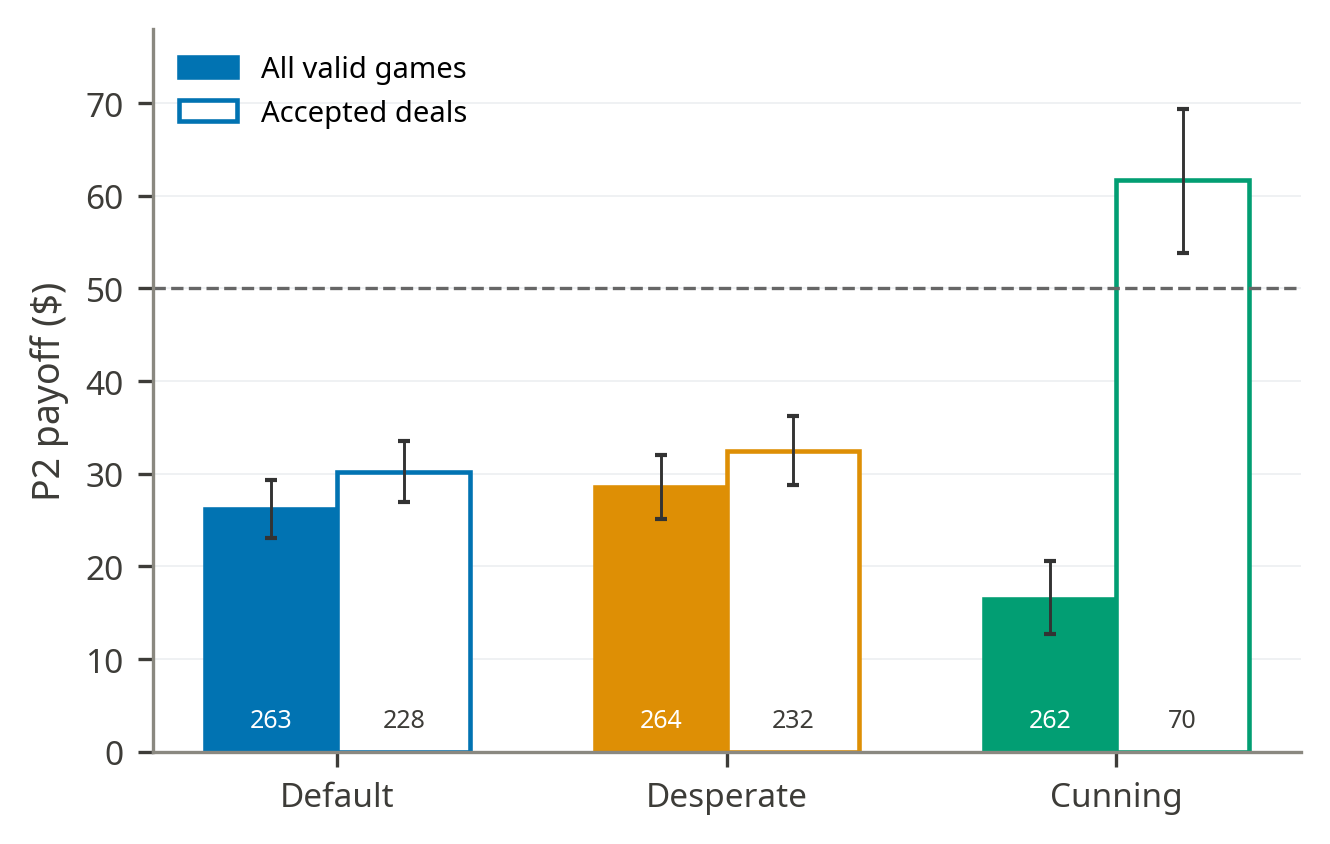
\includegraphics[width=0.8\linewidth]{figures/results/personas/ultimatum_payoff_conditional_deals.png}
    \caption{Mean P2 Ultimatum payoff conditional on reaching a deal, by persona. When a deal does close, the cunning responder keeps far more than the default or desperate responder.}
    \label{fig:persona-payoff-conditional}
\end{figure}

\begin{figure}
    \centering
    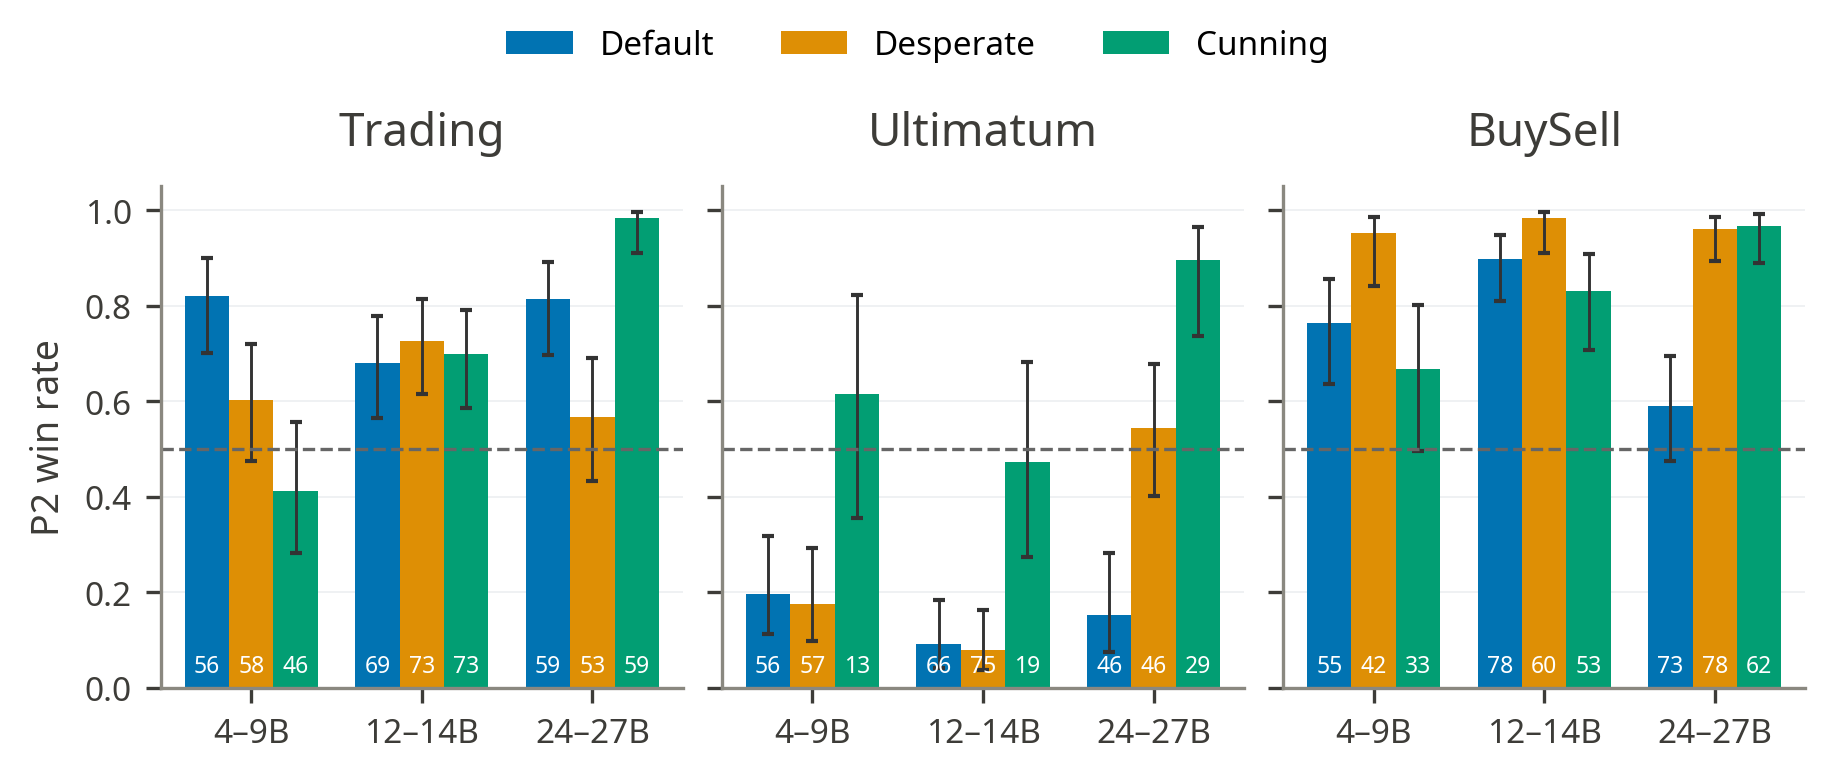
\includegraphics[width=0.8\linewidth]{figures/results/personas/winrate_by_persona_tier.png}
    \caption{P2 win rate by persona, game, and parameter tier under the retry loop. Per-tier decided-game counts are small and the pattern is not monotonic, so tier effects should be read with care.}
    \label{fig:persona-winrate-tier}
\end{figure}

\section{How Personas Reshape Ultimatum Moves} \label{ap4:ultimatum-moves}

Figure~\ref{fig:persona-first-action} decomposes P2's first action, showing how rarely the cunning responder accepts an opening offer. Figure~\ref{fig:persona-rejection-initiator} attributes each no-deal to the side that walked away, and Figure~\ref{fig:persona-nodeal-family} confirms that the elevated cunning no-deal rate is not isolated to one model family.

\begin{figure}
    \centering
    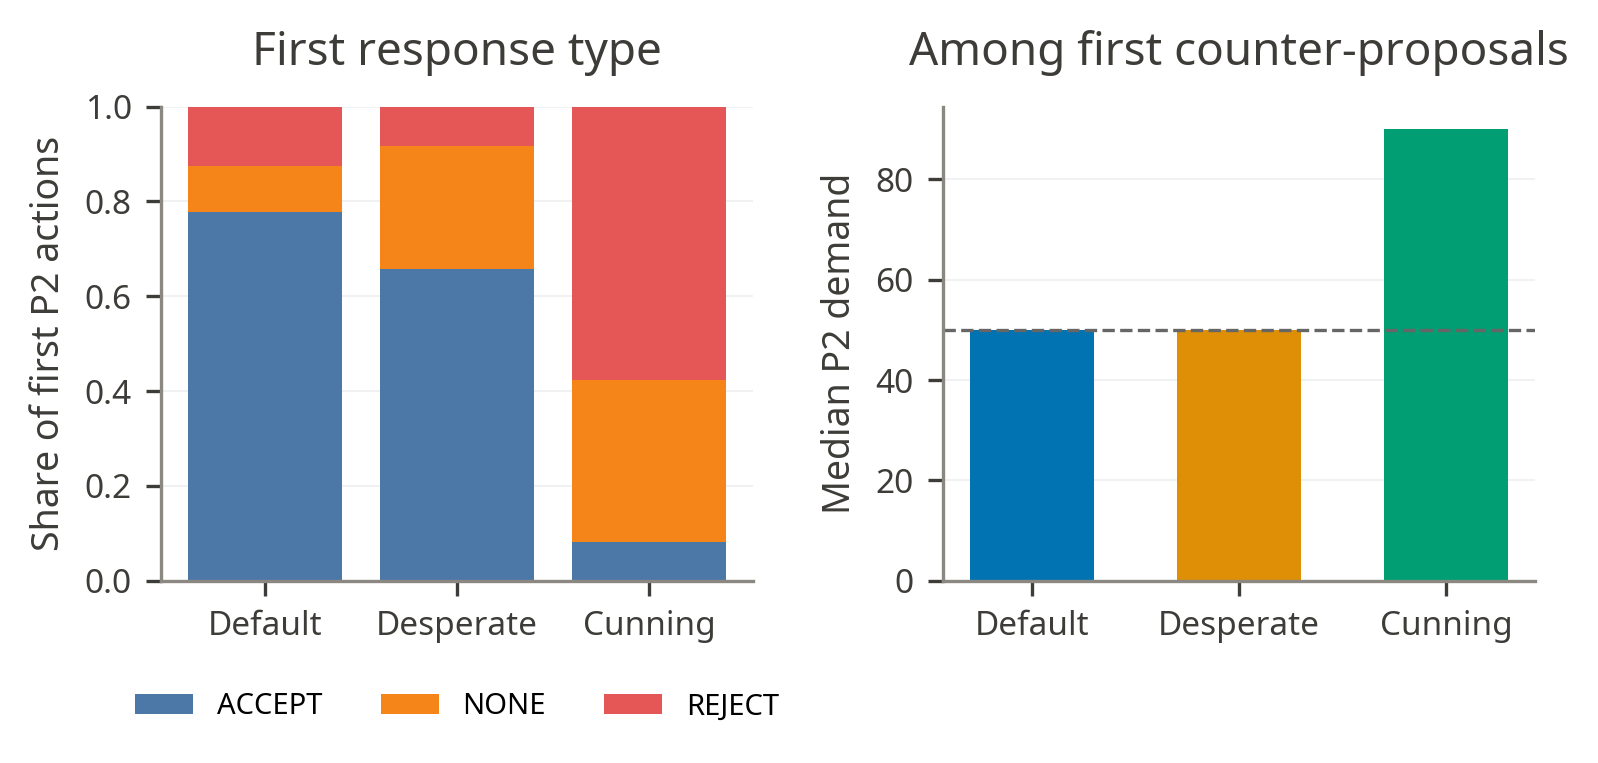
\includegraphics[width=0.8\linewidth]{figures/results/personas/ultimatum_first_p2_action.png}
    \caption{P2's first Ultimatum action by persona: share of opening offers accepted, countered, or rejected outright. The cunning responder accepts only a small fraction and rejects most.}
    \label{fig:persona-first-action}
\end{figure}

\begin{figure}
    \centering
    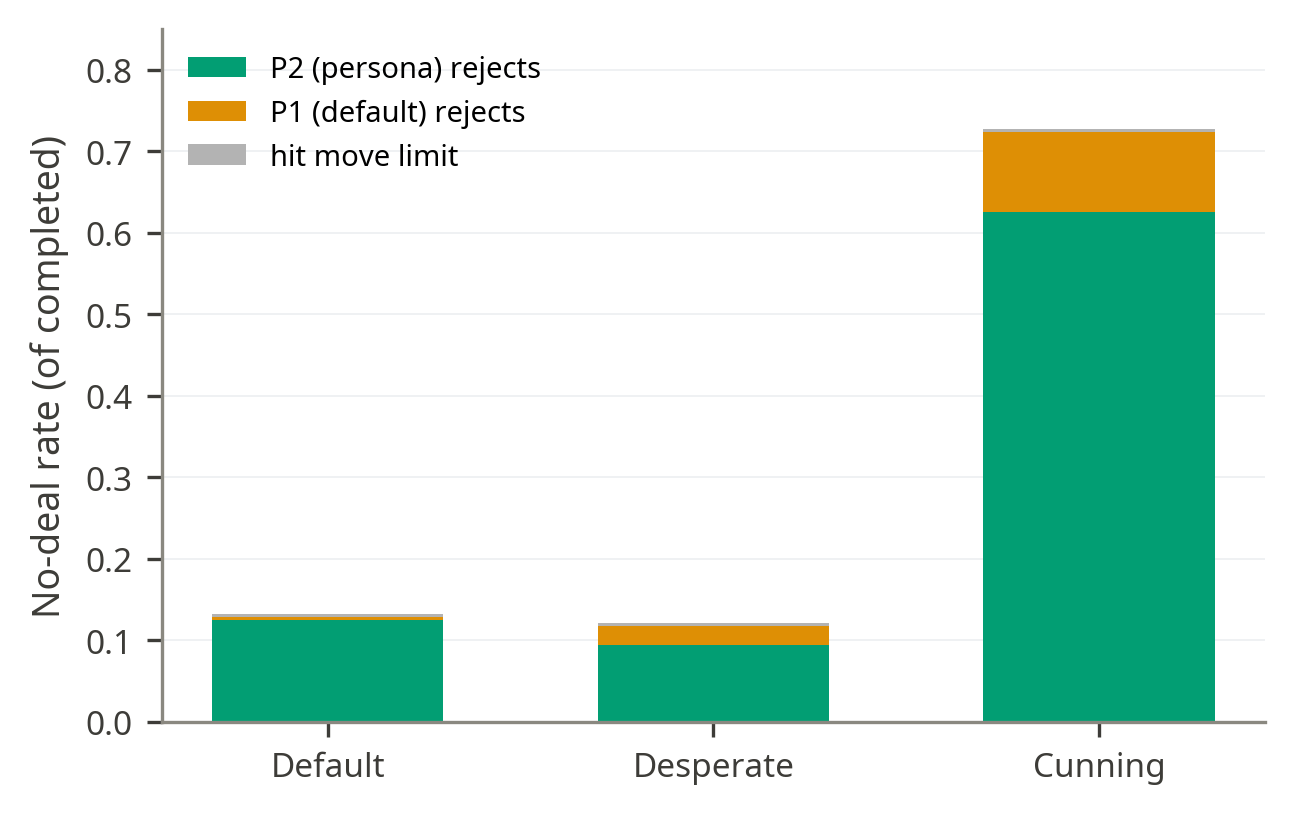
\includegraphics[width=0.8\linewidth]{figures/results/personas/ultimatum_rejection_initiator.png}
    \caption{Initiator of the rejection in no-deal Ultimatum games, by persona. Under cunning, the persona-bearing P2 is responsible for the large majority of the walk-aways.}
    \label{fig:persona-rejection-initiator}
\end{figure}

\begin{figure}
    \centering
    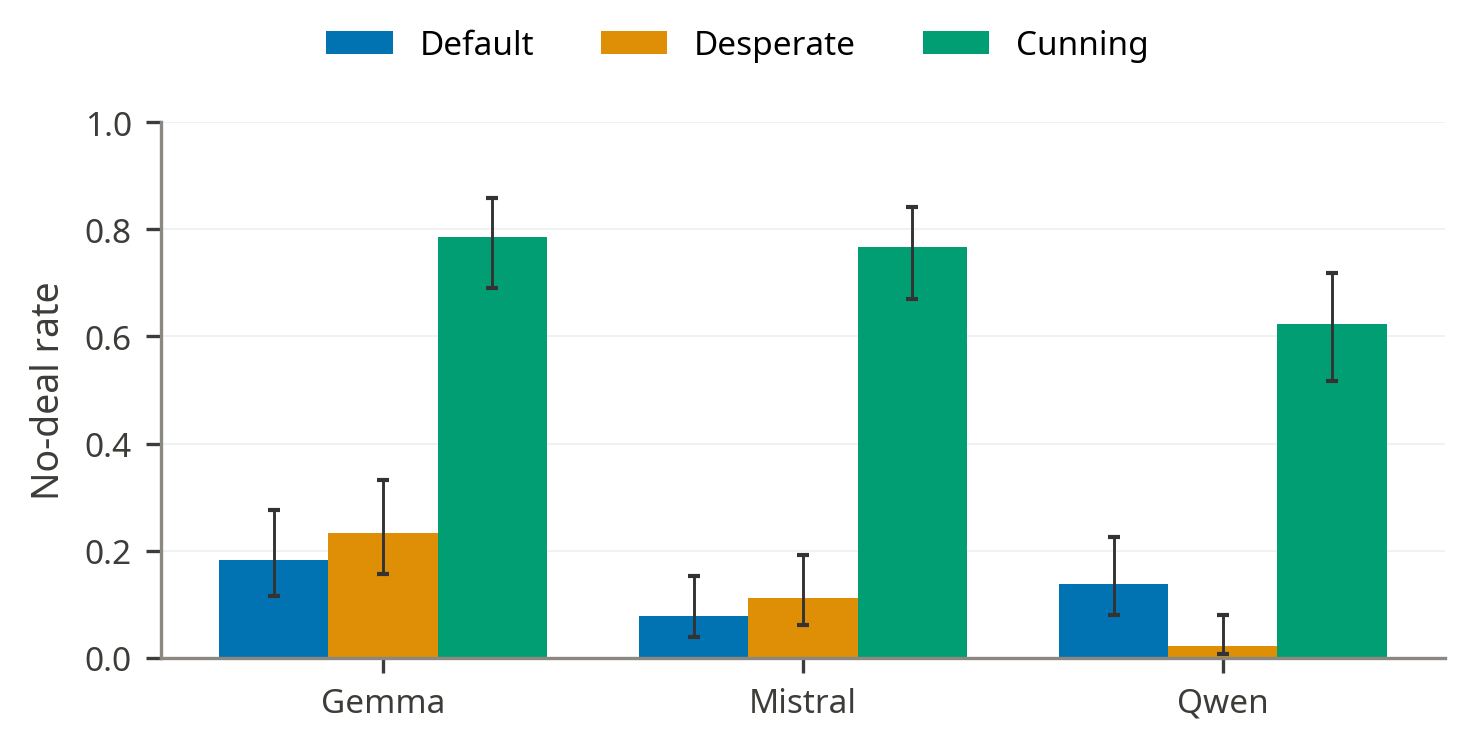
\includegraphics[width=0.8\linewidth]{figures/results/personas/ultimatum_nodeal_family.png}
    \caption{Cunning Ultimatum no-deal rate by responder family. The elevated rate holds across Gemma, Mistral, and Qwen, so it is not an artefact of a single family.}
    \label{fig:persona-nodeal-family}
\end{figure}

\section{BuySell Price Effect} \label{ap4:buysell-price}

Figure~\ref{fig:persona-buysell-price} decomposes the accepted-price distribution by persona.

\begin{figure}
    \centering
    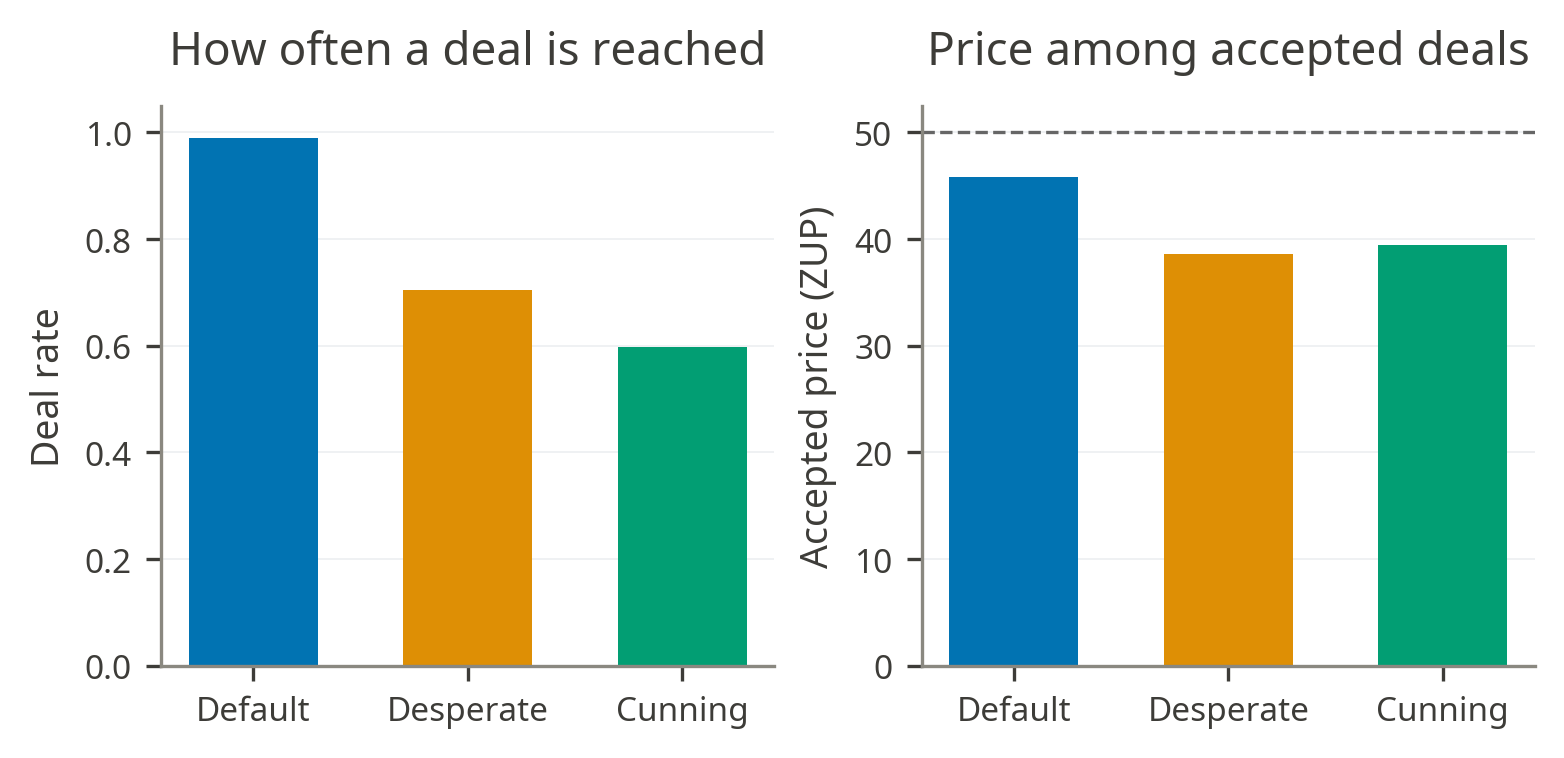
\includegraphics[width=0.8\linewidth]{figures/results/personas/buysell_deal_price_decomposition.png}
    \caption{Accepted BuySell price by persona under the retry loop. The desperate buyer pulls the median accepted price down, raising buyer surplus on the deals that close.}
    \label{fig:persona-buysell-price}
\end{figure}

\section{Per-Model Heterogeneity} \label{ap4:heterogeneity}
 
Figure~\ref{fig:persona-winrate-heatmap} gives the per-model win-rate change for each persona and game, and Figure~\ref{fig:persona-baseline-delta} shows the same effect against each model's default baseline.

\begin{figure}
    \centering
    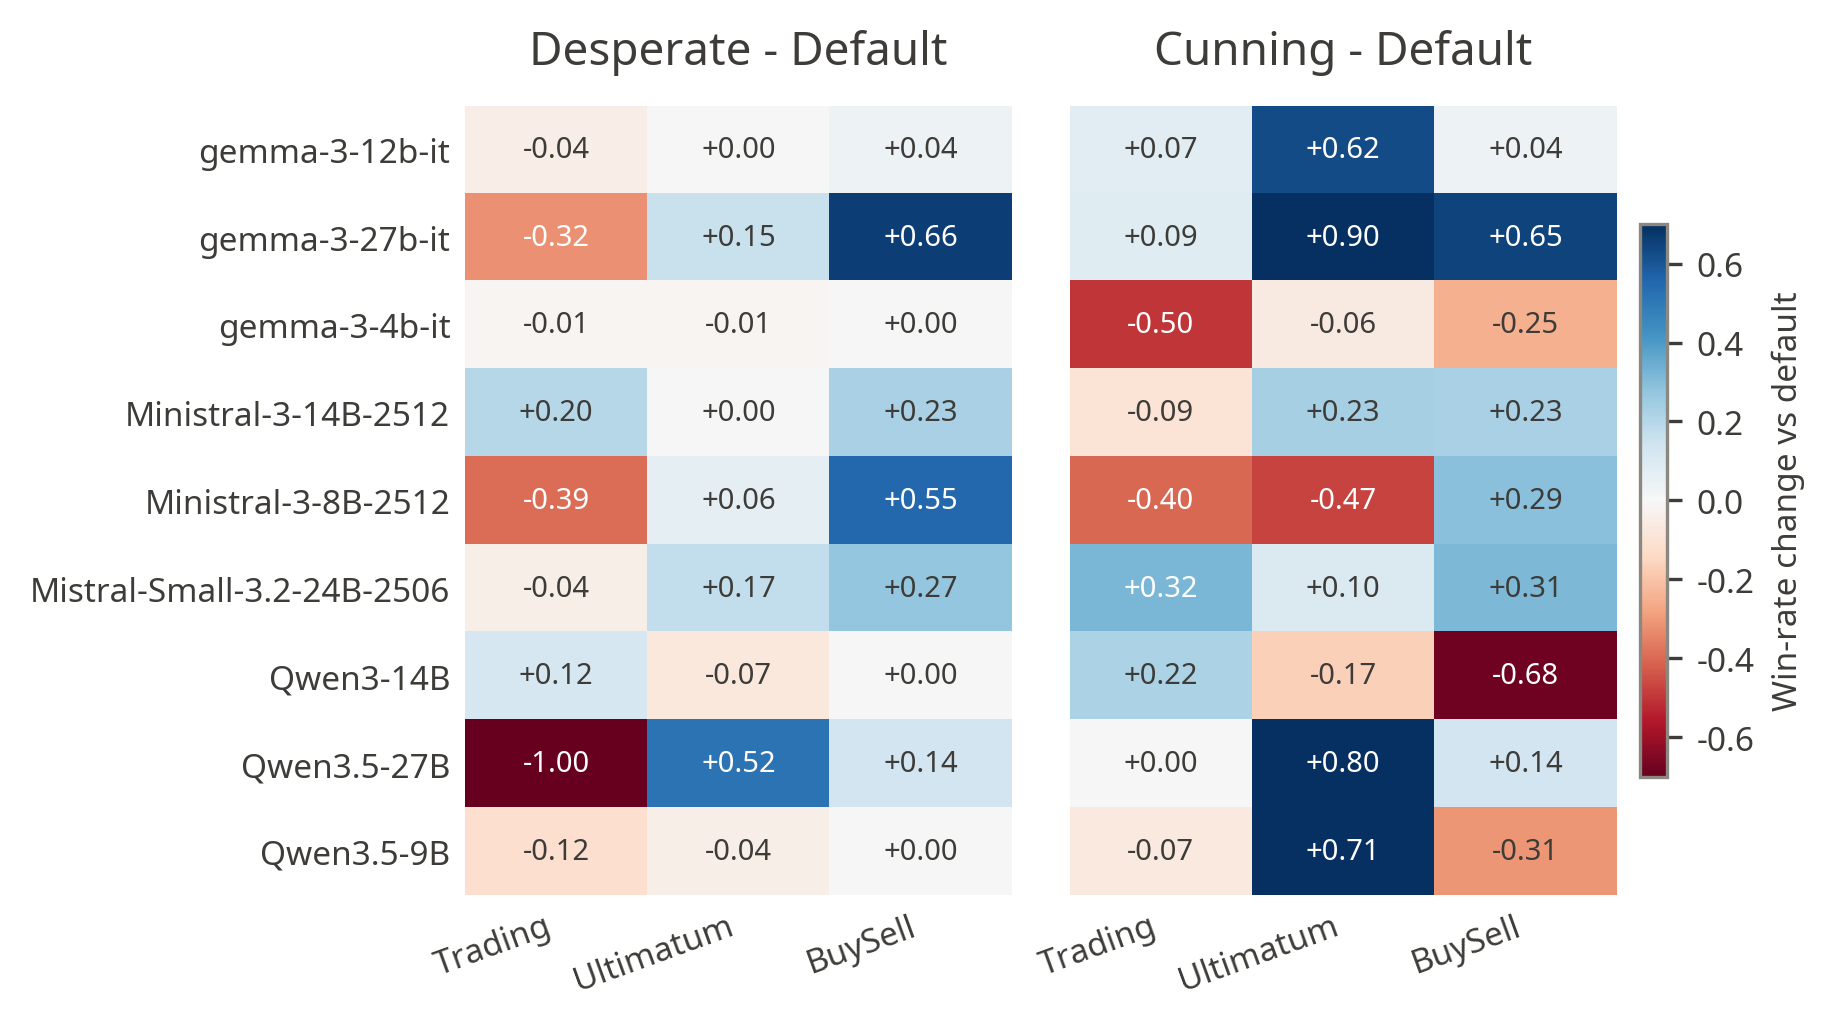
\includegraphics[width=\linewidth]{figures/results/personas/winrate_delta_heatmap.png}
    \caption{Per-model change in P2 win rate relative to the default condition, by persona and game under the retry loop. The effect varies in both size and sign across models.}
    \label{fig:persona-winrate-heatmap}
\end{figure}

\begin{figure}
    \centering
    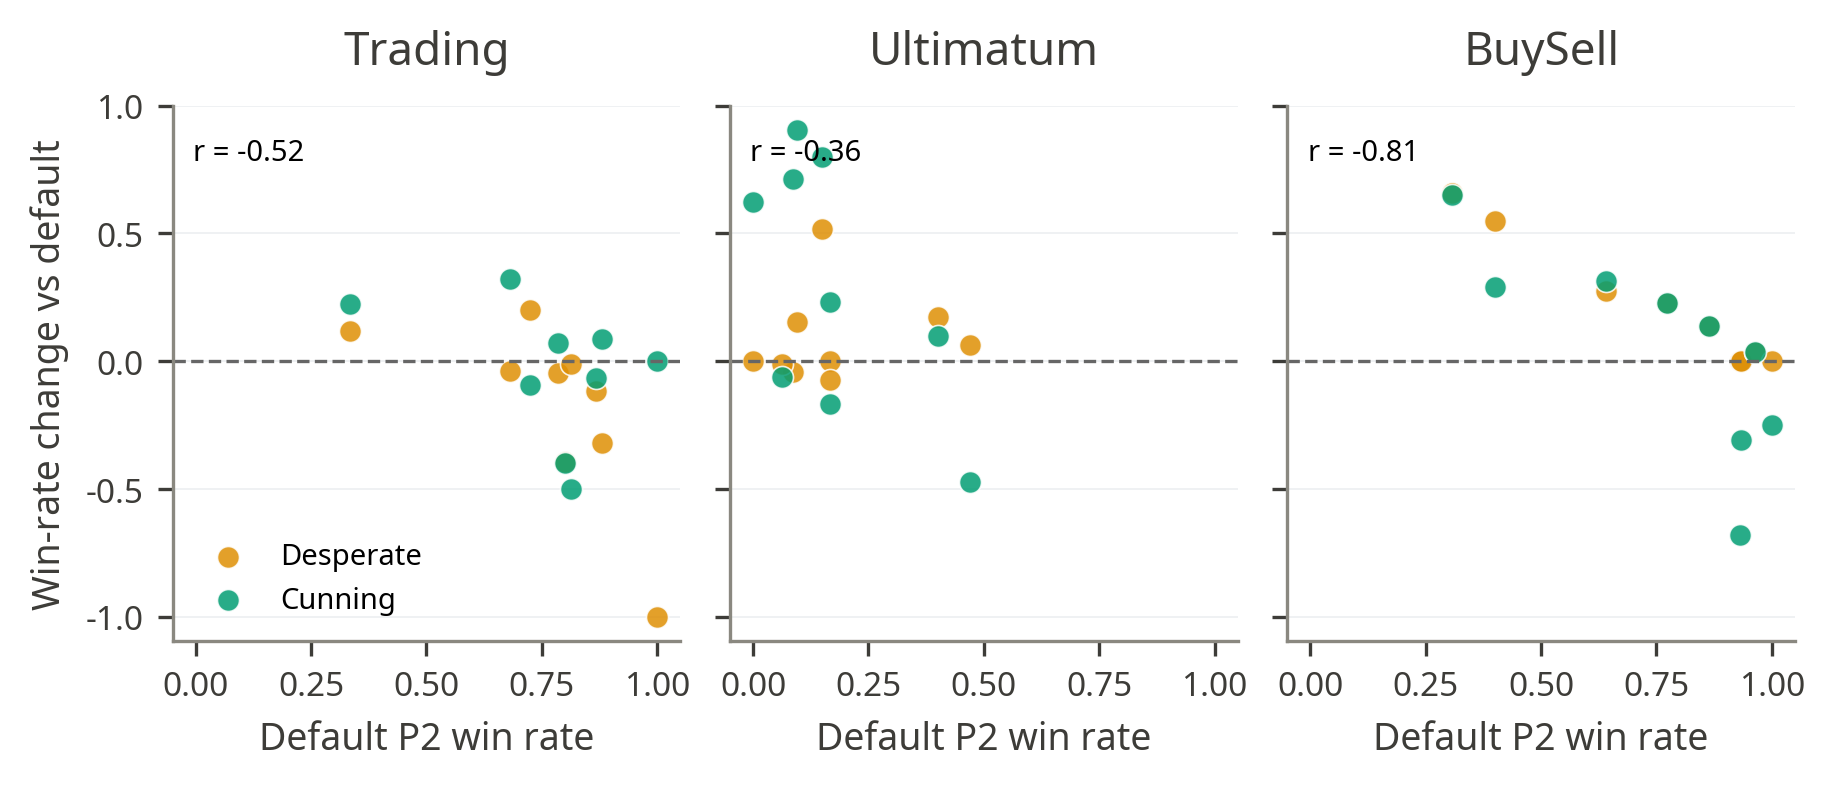
\includegraphics[width=0.8\linewidth]{figures/results/personas/baseline_vs_persona_delta.png}
    \caption{Per-model persona win rate against the model's own default baseline. Points above the diagonal mark models the persona helps; points below mark those it hurts.}
    \label{fig:persona-baseline-delta}
\end{figure}
